\documentclass[11pt]{article}
\usepackage[T1]{fontenc}
\usepackage{textcomp}
\usepackage[utf8]{inputenc}
\usepackage{lmodern}
\usepackage{amsmath,amssymb}
\usepackage{graphicx}
\usepackage{booktabs,array}
\usepackage[round,authoryear]{natbib}
\usepackage[margin=1in]{geometry}
\usepackage{caption}
\usepackage{hyperref}
\usepackage{xurl}
\usepackage{microtype}
\usepackage{fancyvrb}
\usepackage{CJKutf8}
\hypersetup{colorlinks=true,linkcolor=blue,citecolor=blue,urlcolor=blue,pdftitle={Executable Matrix Programs},pdfauthor={Maxim Vladimirovich Zhivotok}}
\urlstyle{same}
\setlength{\emergencystretch}{3em}
\setlength{\parindent}{1.2em}
\setlength{\parskip}{0.25em}
\providecommand{\tightlist}{\setlength{\itemsep}{0pt}\setlength{\parskip}{0pt}}
\title{Executable Matrix Programs: faithful weight-derived replacement and factorized intervention in pretrained transformers}
\author{Maxim Vladimirovich Zhivotok\\\small Independent Researcher, Ukraine\\\small \href{mailto:maxwelhelp@gmail.com}{maxwelhelp@gmail.com}\thanks{Code and results: \url{https://github.com/maxwelhelp/matrix-programs}}}
\date{}
\begin{document}
\begin{CJK*}{UTF8}{gbsn}
\maketitle
\begin{abstract}
We present a method for extracting \textbf{executable component-level matrix programs} from a pretrained decoder-only transformer without retraining or modifying its weights. For RoPE attention, the method constructs a weight-derived QK routing target \(M^{\mathrm{aug}}_{qk}[d]\), indexed by relative distance, and a VO payload map \(C^{\mathrm{aug}}_{vo}\); for a SwiGLU MLP, it constructs an exact atom program with a gate/read/write factorization. Unlike input-specific locally linear representations, these structural objects are derived directly from the weights and reused across inputs. On Qwen2.5-0.5B-Instruct, we simultaneously replace all 336 attention heads and all 24 MLP sublayers with program execution inside the native forward pass. Across 64 prompts, the median relative error of the full logit vector is \textbf{0.258\%}, the 95th percentile is \textbf{0.566\%}, the maximum is \textbf{0.923\%}, and the top-1 prediction is preserved in \textbf{100\%} of cases. Using the same interface, we construct a complete factorized causal atlas: exact replacement, QK-off, and VO-off are measured separately for all 336 heads, while exact replacement and MLP-off are measured for all 24 MLPs. The median ratios of intervention effect to observed replacement discrepancy are \textbf{24.89$\times$} for QK, \textbf{20.62$\times$} for VO, and \textbf{152.05$\times$} for MLPs. Downstream propagation profiles show that, for \textbf{75.0\%} of QK interventions and \textbf{71.4\%} of VO interventions, the peak internal effect occurs at least four layers after the source; the median delays to the peak are \textbf{10} and \textbf{9} layers, respectively. The matrix program therefore serves not only as an analytic description of a component, but as an \textbf{executable interface} for faithful replacement, factorized intervention, and analysis of distributed computation across model depth.
\end{abstract}

\section{Introduction}

Mechanistic interpretability seeks to recover the computational
structure of a trained network: to determine which model components
implement particular transformations and how these transformations
jointly produce an output. Important lines of work for transformers
include QK/OV circuit analysis, activation patching and causal tracing,
sparse autoencoders, input-specific locally linear mappings,
singular-vector decompositions of internal components, and RASP-style
decompilation. A practical question nevertheless remains: can we extract
from the weights of a modern language model an \textbf{explicit and
executable} component program, run it again inside the original forward
pass, and use it to replace not a single selected tensor but the
complete attention+MLP backbone?

Modern decoder transformers make this task more difficult through
implementation details including pre-normalization, RMSNorm, RoPE, GQA,
q/k/v biases, causal masking, gated SwiGLU MLPs, and dtype-dependent
arithmetic. Each element is individually familiar, but a faithful
extractor must align all of them with the native implementation. In this
work, we construct such an extractor for a Qwen2.5-style architecture
and evaluate not only local reconstruction, but also \textbf{global
executable replacement} inside actual inference.

\subsection{Main contributions}

\begin{enumerate}
\def\labelenumi{\arabic{enumi}.}
\item
  \textbf{A unified executable, weight-derived component-program representation.}
  Building on the established QK/OV circuit decomposition and RoPE's
  relative-position formulation~\citep{elhage2021framework,su2021roformer},
  we instantiate a reusable program for the modern
  RoPE/GQA/RMSNorm/bias/SwiGLU stack: relative-distance-indexed
  affine-bilinear QK targets $M^{\mathrm{aug}}_{qk}[d]$, an affine VO map
  $C^{\mathrm{aug}}_{vo}$, and an exact SwiGLU atom program that retains
  the native nonlinearity as input-dependent coefficients over static
  rank-1 atoms with a gate/read/write factorization. The contribution is
  the integrated executable representation and its faithful reinsertion,
  not novelty of the underlying QK/OV decomposition, RoPE identity, or
  algebraic SwiGLU expansion. Unlike input-specific Jacobian mappings
  \citep{golden2025locally}, the structural objects are derived from the
  weights once and reused across inputs; unlike transcoders
  \citep{dunefsky2024transcoders}, no surrogate model is trained.
\item
  \textbf{Global executable replacement.} All 336 attention heads and
  all 24 MLP sublayers of Qwen2.5-0.5B-Instruct are replaced by
  weight-derived program execution inside the native forward pass; the
  complete backbone preserves the top-1 prediction on all 64 prompts
  with a median logit error of \textbf{0.258\%}.
\item
  \textbf{A complete factorized attention causal atlas.} For every head,
  we separately measure exact replacement, QK-off, VO-off, and
  downstream propagation, thereby separating routing from payload.
\item
  \textbf{A complete MLP atlas.} For all 24 MLPs, we measure exact
  replacement and causal removal; intervention effects are two to three
  orders of magnitude larger than the replacement discrepancy.
\item
  \textbf{Effect-to-replacement-discrepancy calibration.} Each
  intervention effect is normalized by the discrepancy of the same
  executable replacement interface---\textbf{24.89$\times$} for QK,
  \textbf{20.62$\times$} for VO, and \textbf{152.05$\times$} for MLPs at
  the median. We use this as a reusable calibration practice for
  separating intervention effects from artifacts of the replacement
  implementation; it is not presented as an independent causal
  identification theorem.
\item
  \textbf{Downstream profiling.} We measure not only the final logit
  effect, but also the change in the residual stream after every
  subsequent layer, exposing delayed and preparatory components. The
  median delays to the peak are 10 layers for QK interventions and 9
  layers for VO interventions.
\item
  \textbf{A verified extractor for a modern stack.} The implementation
  accounts for RoPE, RMSNorm, GQA, q/k/v biases, and SwiGLU and releases
  complete machine-readable reports. A direct control shows that folding
  the learned biases is empirically necessary: the no-bias QK form has a
  median error of \textbf{105\%}, compared with \textbf{0.0526\%} for the
  complete affine form.
\end{enumerate}

Separately, we describe an \textbf{exploratory gate lens}. Because the
activation of a SwiGLU unit is modulated by
$\operatorname{silu}(W_g x)$, we use the gate projection $W_g$ as a
qualitative probe of unit selectivity rather than treating the up
projection $W_u$ alone as the selector. We use this lens only in the
illustrative case study in Section~6.5 and do not treat it as a validated
main contribution pending a quantitative benchmark (Limitation~9).

\subsection{Claims we do not make}

We do not claim novelty for the general QK/OV decomposition, the
algebraic expansion of SwiGLU, homogeneous coordinates as a mathematical
device, the relative-position identity of RoPE, activation ablation in
general, representing a transformer as a matrix system in general,
resolving superposition, or accelerating inference. We also do not claim
universal support for arbitrary architectures without an architecture
adapter.

\section{Architecture and notation}

Consider a decoder-only transformer with residual dimension \(H\). We
denote the state at position \(t\) before a layer component by
\(x_t\in\mathbb{R}^{H}\).

\subsection{RMSNorm}

\[
\widetilde{x} = \operatorname{RMSNorm}_{\gamma}(x) = \frac{x}{\sqrt{\operatorname{mean}(x^2)+\varepsilon}}\odot\gamma.
\]

\subsection{Homogeneous
coordinates}

For an affine projection \(z=Wx+b\), define

\[
x_{\mathrm{aug}}=\begin{bmatrix}x\\1\end{bmatrix},\qquad W_{\mathrm{aug}}=\begin{bmatrix}W & b\end{bmatrix},
\]

so that \(z=W_{\mathrm{aug}}x_{\mathrm{aug}}\). In a companion
reconstruction run, the QK form with folded biases had a median error of
\textbf{0.0526\%}, whereas the no-bias control had an error of
\textbf{105\%}. For Qwen2.5, homogeneous coordinates are therefore a
necessary part of the faithful circuit target rather than a cosmetic
notation.

\subsection{RoPE convention}

In the implementation, tensors are stored as row vectors and RoPE is
applied as \(vR_p^\top\). The formulas below use the equivalent
column-vector convention. The matrix ordering is validated by direct
reconstruction against the native forward pass.

\section{Weight-derived component programs}

\subsection{QK: routing program}

For an attention head of dimension \(D\),

\[
q_i^{\mathrm{pre}} = W_q\widetilde{x}_i+b_q,\qquad k_j^{\mathrm{pre}} = W_k\widetilde{x}_j+b_k.
\]

After RoPE~\citep{su2021roformer},

\[
q_i=R_iq_i^{\mathrm{pre}},\qquad k_j=R_jk_j^{\mathrm{pre}}.
\]

The pre-softmax score is

\[
s_{ij}=\frac{q_i^\top k_j}{\sqrt{D}} = x_{\mathrm{aug},i}^{\top} M^{\mathrm{aug}}_{qk}[i-j] x_{\mathrm{aug},j},
\]

where

\[
M^{\mathrm{aug}}_{qk}[d] = \frac{(W_q^{\mathrm{aug}})^\top R_{\mathrm{rel}}[d] W_k^{\mathrm{aug}}}{\sqrt{D}}.
\]

At runtime, the same program can be executed in factorized form through
augmented q and k vectors, without necessarily materializing a full
\((H+1)\times(H+1)\) matrix for every distance.

\subsection{VO: payload program}

\[
C^{\mathrm{aug}}_{vo}=W_oW_v^{\mathrm{aug}},\qquad \operatorname{payload}_j=C^{\mathrm{aug}}_{vo}x_{\mathrm{aug},j},
\]

\[
y_i=\sum_j A_{ij}\operatorname{payload}_j.
\]

QK determines routing, whereas VO determines the transported content and
its write direction.

\subsection{SwiGLU MLP}

\[
y=W_d\left[\operatorname{silu}(W_g\widetilde{x})\odot (W_u\widetilde{x})\right].
\]

Component-wise,

\[
y=\sum_{j=1}^{m} a_j(x)W_d[:,j],\qquad a_j(x)=\operatorname{silu}(W_{g,j}\widetilde{x})\cdot (W_{u,j}\widetilde{x}).
\]

We factor each neuron into gate, read, and write terms:

\[
\operatorname{gate}_j(x)=\operatorname{silu}(W_{g,j}\widetilde{x}),\quad
\operatorname{read}_j(x)=W_{u,j}\widetilde{x},\quad
\operatorname{write}_j=W_d[:,j],
\]

and define the static rank-1 atom

\[
B_j = W_d[:,j]\otimes W_u[j,:].
\]

\section{Executable replacement and factorized interventions}

For a selected set of attention heads \(S_L\) in layer \(L\), we compute
the native contribution \(Y^{\mathrm{native}}_{S_L}\) and the program
contribution \(Y^{\mathrm{program}}_{S_L}\). The attention module output
is replaced by

\[
Y^{\mathrm{patched}} = Y^{\mathrm{module}} - Y^{\mathrm{native}}_{S_L} + Y^{\mathrm{program}}_{S_L}.
\]

For an MLP, the native output is replaced by

\[
Y^{\mathrm{program}}_{\mathrm{MLP}} = \sum_j a_j(x)W_d[:,j].
\]

The global experiment installs hooks on all 24 attention sublayers and
all 24 MLP sublayers simultaneously, thereby replacing the complete
attention+MLP backbone. Layer norms, embeddings, residual additions, and
the language-model head remain native.

The interventions are defined as follows:

\begin{itemize}
\tightlist
\item
  \textbf{QK-off:} content-dependent QK scores for the selected head are
  zeroed before softmax.
\item
  \textbf{VO-off:} the selected head's payload is zeroed while its
  routing computation is retained.
\item
  \textbf{MLP-off:} the selected MLP output is zeroed.
\end{itemize}

The main exact-replacement metric is

\[
E_{\mathrm{logit}} = 100\cdot \frac{\|\ell_{\mathrm{patched}}-\ell_{\mathrm{base}}\|_2}{\|\ell_{\mathrm{base}}\|_2}.
\]

We also measure KL divergence, Jensen-Shannon divergence, logit cosine
similarity, top-1 preservation, and top-5 overlap.

Throughout the paper, we use the term \textbf{replacement discrepancy}.
The native identity control in the current implementation is a sanity
check and is not used as an independent estimate of a numerical lower
bound. Per-experiment summaries over prompts use the released
\texttt{torch.median} aggregation, which returns the lower middle value
for an even sample count. Medians reported across rows of the released
head and MLP atlas tables use the conventional median, averaging the two
middle values when the number of components is even.

\section{Experimental setup}

\subsection{Model}

\texttt{Qwen/Qwen2.5-0.5B-Instruct}~\citep{qwen2024technical}:

\begin{itemize}
\tightlist
\item
  24 layers;
\item
  14 attention heads per layer (336 total);
\item
  2 KV heads;
\item
  residual dimension \(H=896\);
\item
  head dimension \(D=64\);
\item
  SwiGLU intermediate dimension \(m=4864\);
\item
  fp16;
\item
  eager attention.
\end{itemize}

\subsection{Prompt suite}

The suite contains 64 short next-token prompts:

\begin{itemize}
\tightlist
\item
  Capitals: 12
\item
  Factual: 12
\item
  Math: 10
\item
  Code: 10
\item
  Continuation: 10
\item
  Russian: 4
\item
  Ukrainian: 4
\item
  German: 1
\item
  Spanish: 1
\end{itemize}

\subsection{Experimental scale}

\begin{itemize}
\tightlist
\item
  1,662 main experiments;
\item
  106,368 experiment-prompt evaluations;
\item
  global replacements;
\item
  a complete 336-head atlas;
\item
  a complete 24-MLP atlas;
\item
  24 layer-group profiles;
\item
  downstream propagation profiles.
\end{itemize}

\subsection{Reproducibility}

The arXiv repository records:

\begin{itemize}
\tightlist
\item
  the \texttt{torch} and \texttt{transformers} versions;
\item
  the revision of \texttt{Qwen/Qwen2.5-0.5B-Instruct};
\item
  the random seed;
\item
  hardware: \textbf{Tesla P40 24GB};
\item
  the wall-clock time of the full run;
\item
  exact commands;
\item
  the SHA256 hash of the main script;
\item
  the corrected atom-split script with independent random seeds.
\end{itemize}

\section{Results}

\subsection{Companion
reconstruction}

\begin{center}
\small
\begin{tabular}{@{}lr@{}}
\toprule
Component & Median relative error \\
\midrule
QK scores with RoPE+bias & 0.0526\% \\
Attention probabilities & 0.0599\% \\
VO head output & 0.0277\% \\
MLP output & 0.0426\% \\
QK without bias folding & 105\% \\
\bottomrule
\end{tabular}
\end{center}

The no-bias control shows that, for Qwen2.5, folding biases through
homogeneous coordinates is necessary rather than cosmetic.

\subsection{Global executable
replacement}

\begin{table}[t]
\centering
\small
\begin{tabular}{lrrrrrr}
\toprule
Replacement & N & Median & p95 & Max & Median KL & Top-1 \\
\midrule
All attention & 64 & 0.254\% & 0.477\% & 0.885\% & 3.38e-5 & 100\% \\
All MLPs & 64 & 0.241\% & 0.419\% & 0.883\% & 2.68e-5 & 100\% \\
Attention + MLP & 64 & \textbf{0.258\%} & \textbf{0.566\%} & \textbf{0.923\%} & \textbf{3.09e-5} & \textbf{100\%} \\
\bottomrule
\end{tabular}
\end{table}

Figure~\ref{fig:method} summarizes the method, and Figure~\ref{fig:prompt-suites} reports the category-wise replacement errors. For the complete backbone, the median logit cosine similarity is
\textbf{0.999990}, and the median top-5 overlap is \textbf{1.0}.

\begin{figure}[t]
\centering
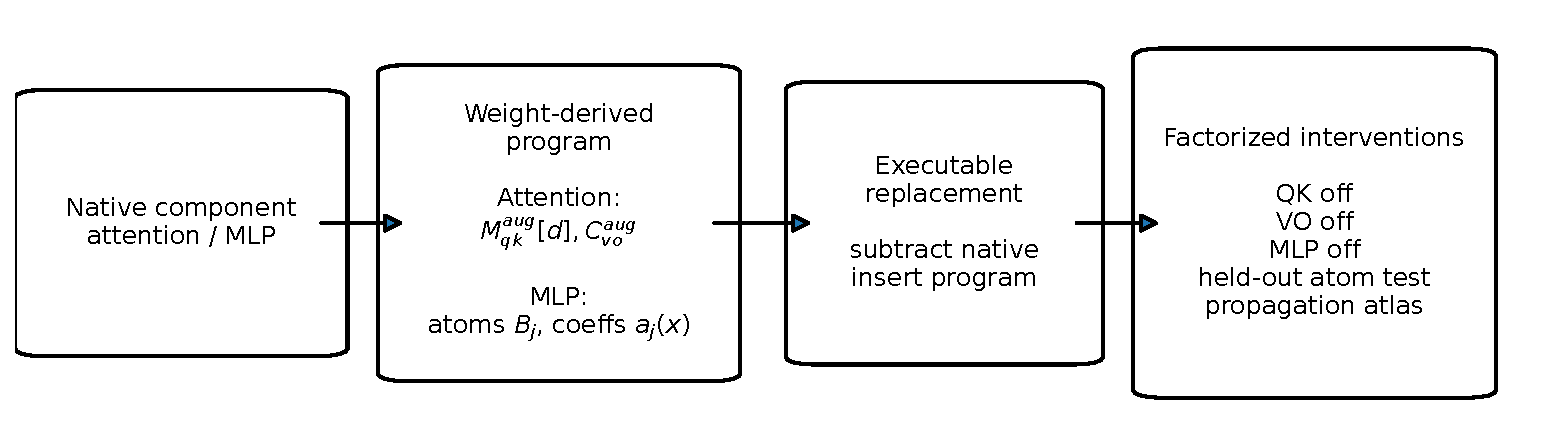
\includegraphics[width=\linewidth]{figures/fig1_method_overview.pdf}
\caption{Extraction of a weight-derived program, its executable replacement inside the native forward pass, and factorized interventions.}
\label{fig:method}
\end{figure}
\subsection{Single-component executable replacement across the
full
model}

\begin{center}
\small
\setlength{\tabcolsep}{3.5pt}
\begin{tabular}{@{}lccccc@{}}
\toprule
Object & \shortstack{Number of\\components} & \shortstack{Median replacement\\discrepancy} & p95 & Max & \shortstack{Aggregate top-1\\preservation} \\
\midrule
Attention head & 336 & 0.137\% & 0.201\% & 0.265\% & 100\% \\
MLP layer & 24 & 0.139\% & 0.192\% & 0.243\% & 99.935\% \\
Full transformer layer & 24 & 0.139\% & 0.214\% & 0.241\% & $>99.9\%$ \\
\bottomrule
\end{tabular}
\end{center}

\subsection{Complete head atlas}

\begin{center}
\small
\begin{tabular}{@{}lrr@{}}
\toprule
Metric & QK-off & VO-off \\
\midrule
Median logit effect & 3.280\% & 2.883\% \\
p95 & 6.859\% & 6.664\% \\
Max & 23.649\% & 11.403\% \\
Median effect/replacement ratio & 24.89$\times$ & 20.62$\times$ \\
Heads with ratio $>10\times$ & 92.86\% & 84.23\% \\
Aggregate top-1 change & 6.12\% & 5.82\% \\
Heads changing top-1 at least once & 96.13\% & 92.56\% \\
\bottomrule
\end{tabular}
\end{center}

\begin{figure}[t]
\centering
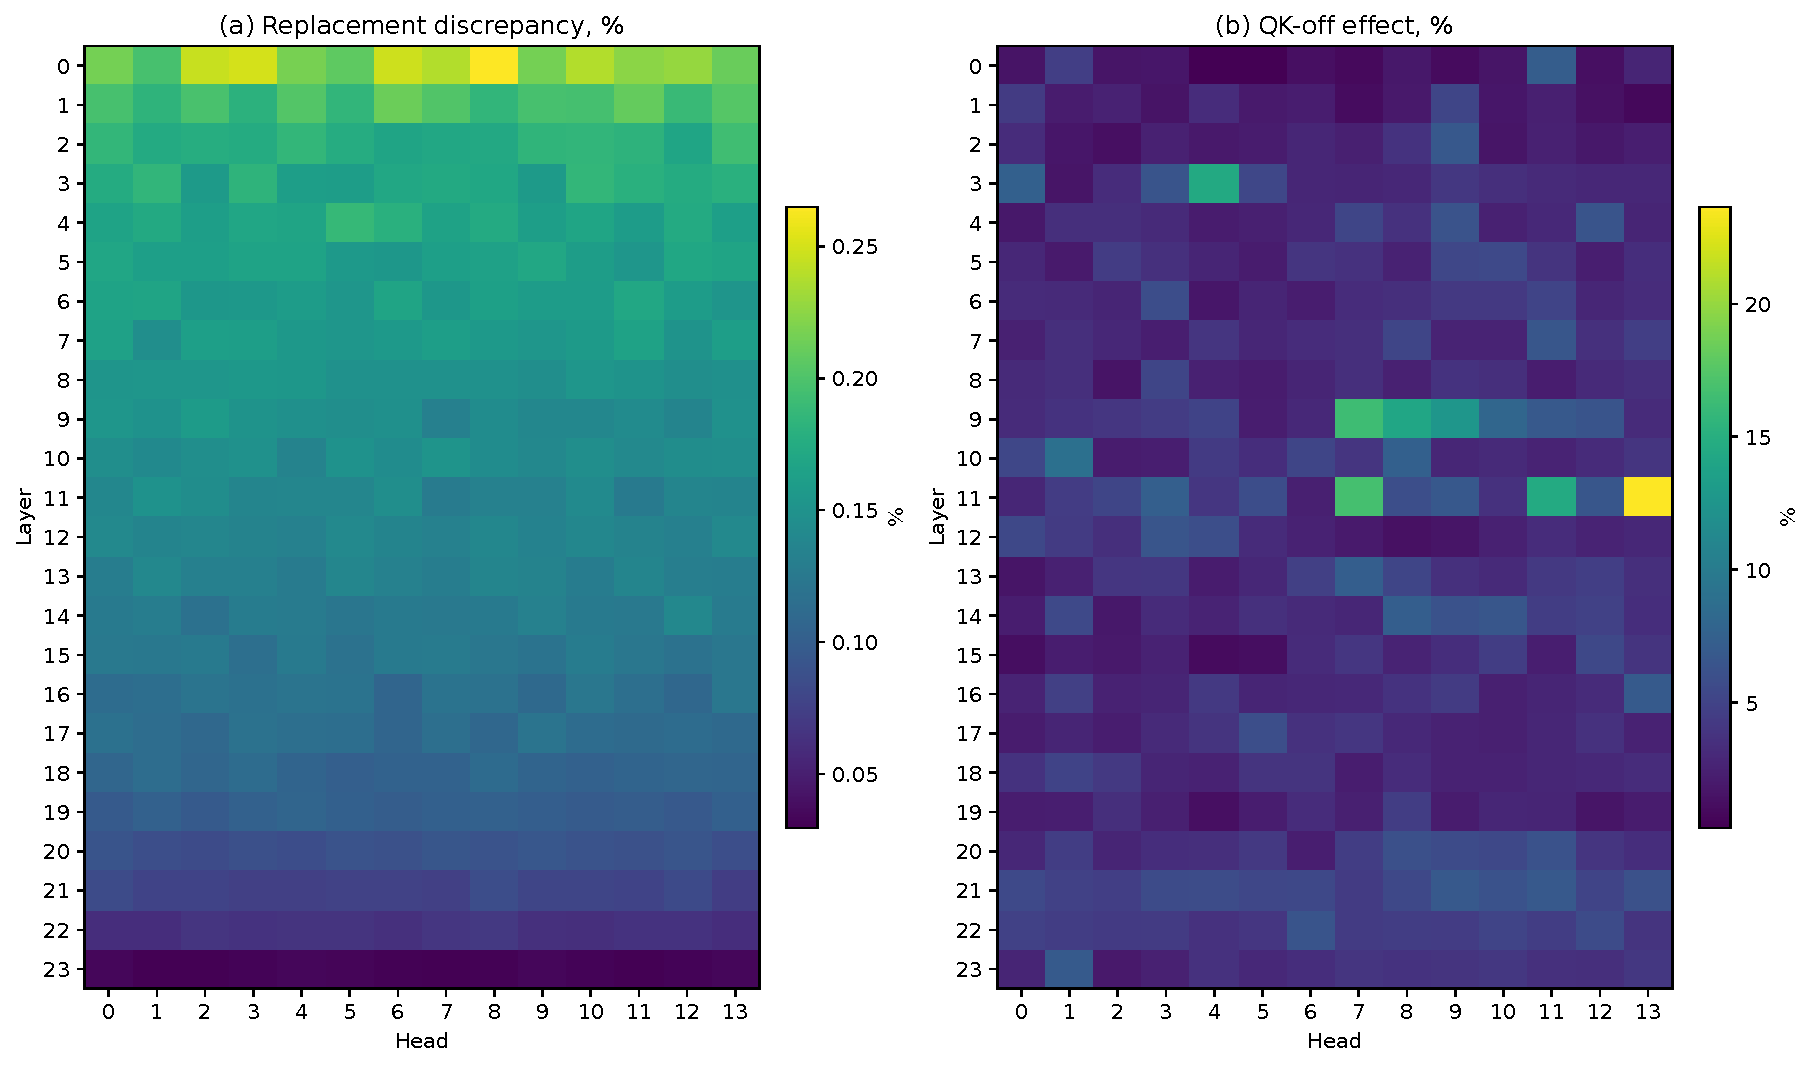
\includegraphics[width=\linewidth]{figures/fig2_head_heatmaps.pdf}
\caption{Complete $24\times14$ atlas. Left: observed replacement discrepancy for each head. Right: QK-off effect for the same head.}
\label{fig:head-atlas}
\end{figure}
\subsection{Qualitative illustration: \texttt{The capital of France is}}

\textbf{This section is illustrative and is not part of the main claims.
The gate lens remains an exploratory tool (see Limitations).}
Nevertheless, a mechanistic-interpretability paper benefits from showing
how the executable interface makes a concrete computation legible.

The prompt \texttt{"The\ capital\ of\ France\ is"} produces the
prediction \texttt{"\ Paris"}. In late layers, the extracted program
exposes three levels of structure.

\textbf{Attention: which heads contribute most and where they read
from.}

\begin{itemize}
\tightlist
\item
  \textbf{L21H6:} contribution \texttt{+1.094}; sources:
  \texttt{\textquotesingle{}France\textquotesingle{}\ (A=0.73)},
  \texttt{\textquotesingle{}The\textquotesingle{}\ (0.15)},
  \texttt{\textquotesingle{}is\textquotesingle{}\ (0.07)}.
\item
  \textbf{L21H1:} contribution \texttt{+0.279}; sources:
  \texttt{\textquotesingle{}France\textquotesingle{}\ (0.41)},
  \texttt{\textquotesingle{}The\textquotesingle{}\ (0.36)}.
\item
  \textbf{L20H5:} contribution \texttt{+0.201}; sources:
  \texttt{\textquotesingle{}France\textquotesingle{}\ (0.52)},
  \texttt{\textquotesingle{}The\textquotesingle{}\ (0.38)},
  \texttt{\textquotesingle{}capital\textquotesingle{}\ (0.05)}.
\end{itemize}

This makes explicit not only the routing, but also the payload, because
the transported content is given by the map
\(C_{vo}^{aug}x_{\mathrm{aug},j}\).

\textbf{MLP atoms: which late-layer atoms are active and what themes
they carry.}

\begin{itemize}
\tightlist
\item
  \textbf{L18 n3178:} \texttt{a=-18.25}; gate lens:
  \texttt{towns,\ hom}.
\item
  \textbf{L20 n4520:} \texttt{a=-30.43}; gate lens:
  \texttt{city,\ .city,\ \_city}.
\item
  \textbf{L20 n3433:} \texttt{a=-9.28}; reads:
  \texttt{congressional,\ 白宫,\ 政府}; writes:
  \texttt{Washington,\ DC,\ 华盛顿}.
\item
  \textbf{L21 n4090:} \texttt{a=+30.97}; reads:
  \texttt{法国,\ French,\ France}; writes:
  \texttt{法国,\ French,\ France}.
\item
  \textbf{L22 n2750:} \texttt{a=-6.73}; reads:
  \texttt{French,\ Prix,\ 法国}; writes: \texttt{巴黎,\ Jean,\ Paris}.
\item
  \textbf{L23 n1465:} \texttt{a=+47.10}; reads:
  \texttt{French,\ France,\ 法国,\ Paris}.
\end{itemize}

Illustratively, these atoms form a semantic chain
\texttt{towns\ $\rightarrow$\ city\ $\rightarrow$\ France\ $\rightarrow$\ Paris}.

\textbf{Causal verification from the earlier exploratory run.}

\begin{itemize}
\tightlist
\item
  \textbf{L23 n1465:} \texttt{$\Delta$logit(real)\ =\ -8.406};
  \texttt{real/random\ =\ 76.9}; \texttt{real/unrelated\ =\ 7.0}.
\item
  \textbf{L21 n4090:} \texttt{$\Delta$logit(real)\ =\ +0.719};
  \texttt{real/random\ =\ 3.5}; \texttt{real/unrelated\ =\ 3.1}.
\end{itemize}

Because the held-out atom suite in the current archive was affected by a
random-control seed bug, this example should be treated as a qualitative
illustration rather than part of the central quantitative result.

\subsection{Complete MLP atlas}

\begin{center}
\small
\begin{tabular}{@{}lr@{}}
\toprule
Metric & Value \\
\midrule
Median replacement discrepancy & 0.139\% \\
Median MLP-off effect & 23.44\% \\
p95 MLP-off & 81.97\% \\
Max MLP-off & 99.51\% \\
Median effect/replacement ratio & 152.05$\times$ \\
Aggregate top-1 change & 38.15\% \\
\bottomrule
\end{tabular}
\end{center}

\subsection{Layer-group
interventions}

\begin{center}
\small
\begin{tabular}{@{}lrr@{}}
\toprule
Intervention & Median logit effect & Median top-1 change rate \\
\midrule
QK off for all heads in the layer & 13.91\% & 17.19\% \\
VO off for all heads in the layer & 10.05\% & 18.75\% \\
MLP off & 23.44\% & 33.59\% \\
VO + MLP off & 27.44\% & 36.72\% \\
\bottomrule
\end{tabular}
\end{center}

\subsection{Downstream propagation and preparatory
components}

\begin{center}
\small
\begin{tabular}{@{}lrr@{}}
\toprule
Statistic & QK & VO \\
\midrule
Median delay to peak & 10 & 9 \\
Peak delayed $\geq 4$ layers & 75.0\% & 71.4\% \\
Median peak/first amplification & 17.98$\times$ & 17.19$\times$ \\
Amplification $>10\times$ & 76.2\% & 73.5\% \\
\bottomrule
\end{tabular}
\end{center}

This section and Figure 3 use the same metric,
\texttt{valid\_tensor\_rel\_percent}: the relative L2 perturbation of
the complete valid residual tensor over the batch of 64 prompts. The
horizontal axis in Figure 3a is aligned to the first residual state
after the source head: \texttt{target\_index\ --\ (source\_layer\ +\ 1)}.

Preparatory examples:

\begin{itemize}
\tightlist
\item
  \textbf{QK L2H5:} final logits \texttt{2.10\%}; first post-source
  residual \texttt{3.53\%}; peak residual \texttt{20.29\%} at target
  residual index \texttt{22}, i.e.~\texttt{19} layers after the first
  post-source residual; internal/final ratio \texttt{9.64$\times$}.
\item
  \textbf{QK L17H2:} final logits \texttt{2.13\%}; first post-source
  residual \texttt{0.219\%}; peak residual \texttt{5.59\%} at target
  residual index \texttt{23}, i.e.~a delay of \texttt{5} layers;
  amplification \texttt{25.57$\times$}.
\item
  \textbf{VO L16H10:} final logits \texttt{2.14\%}; first post-source
  residual \texttt{0.378\%}; peak residual \texttt{5.78\%} at target
  residual index \texttt{23}, i.e.~a delay of \texttt{6} layers;
  amplification \texttt{15.31$\times$}.
\end{itemize}

\begin{figure}[t]
\centering
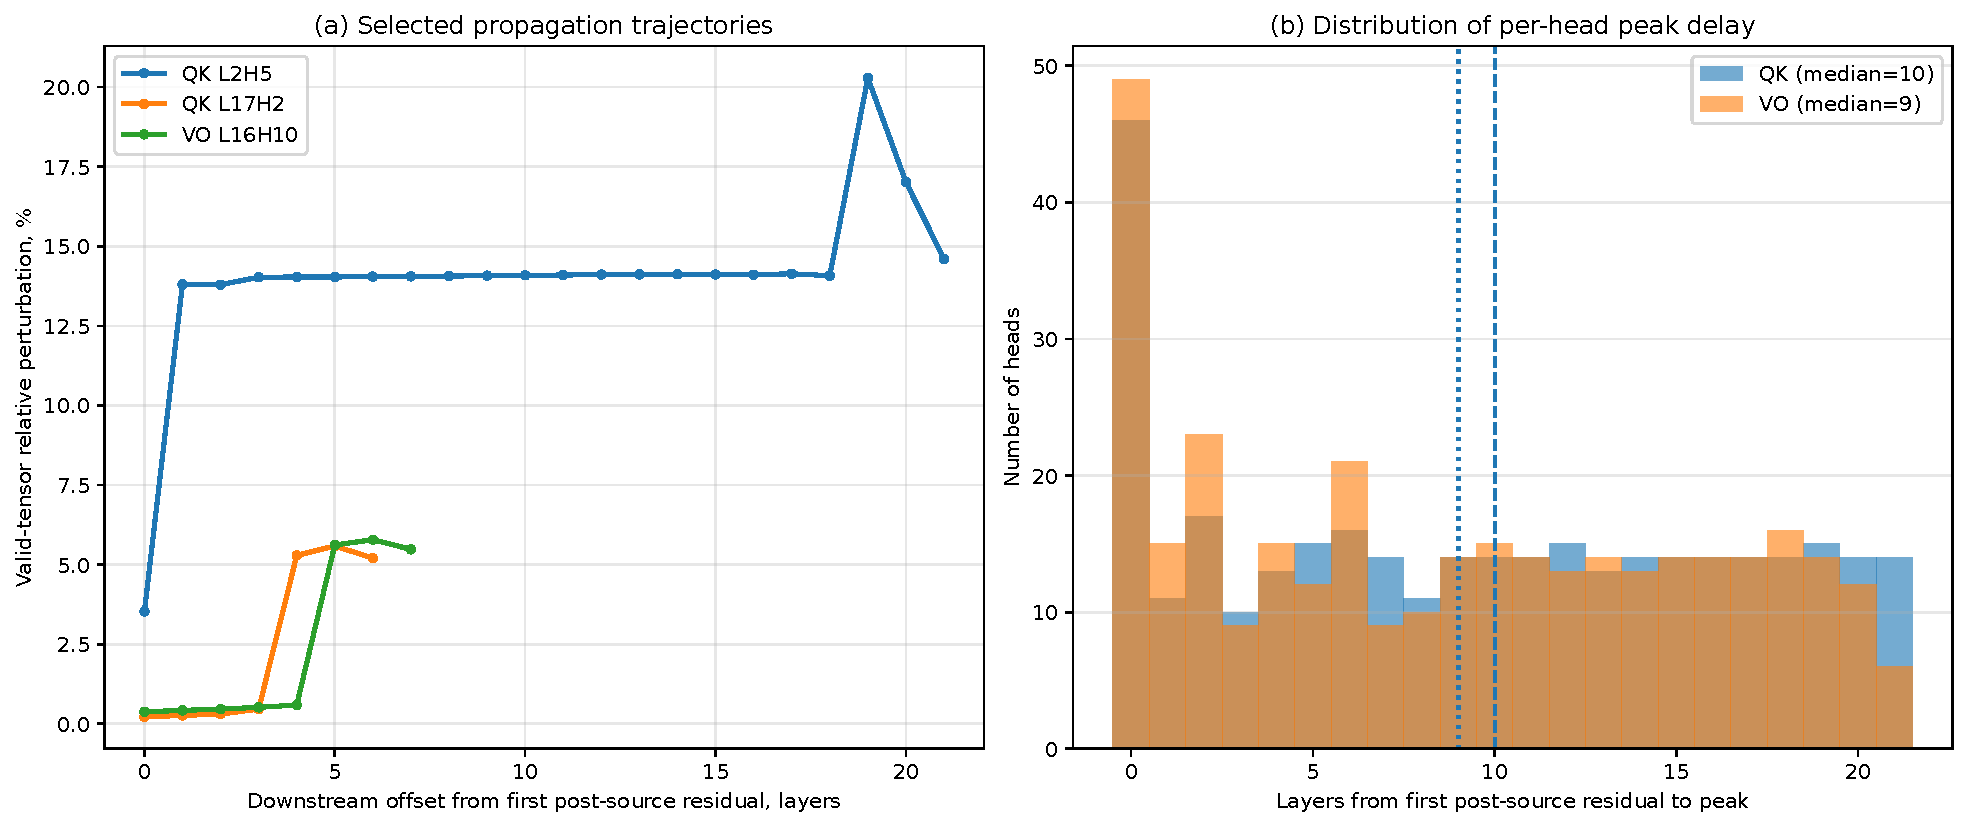
\includegraphics[width=\linewidth]{figures/fig3_propagation_profiles.pdf}
\caption{(a) Selected propagation trajectories computed with \texttt{valid\_tensor\_rel\_percent} and aligned to the first post-source residual. (b) Distribution of the per-head delay to the maximum valid-tensor perturbation; medians are 10 layers for QK and 9 layers for VO.}
\label{fig:propagation}
\end{figure}

Figure~\ref{fig:propagation} visualizes the same metric. These results support the conclusion that a weak direct final-logit
effect does not imply a small computational role: many heads prepare
states that are used by subsequent layers.

\begin{figure}[t]
\centering
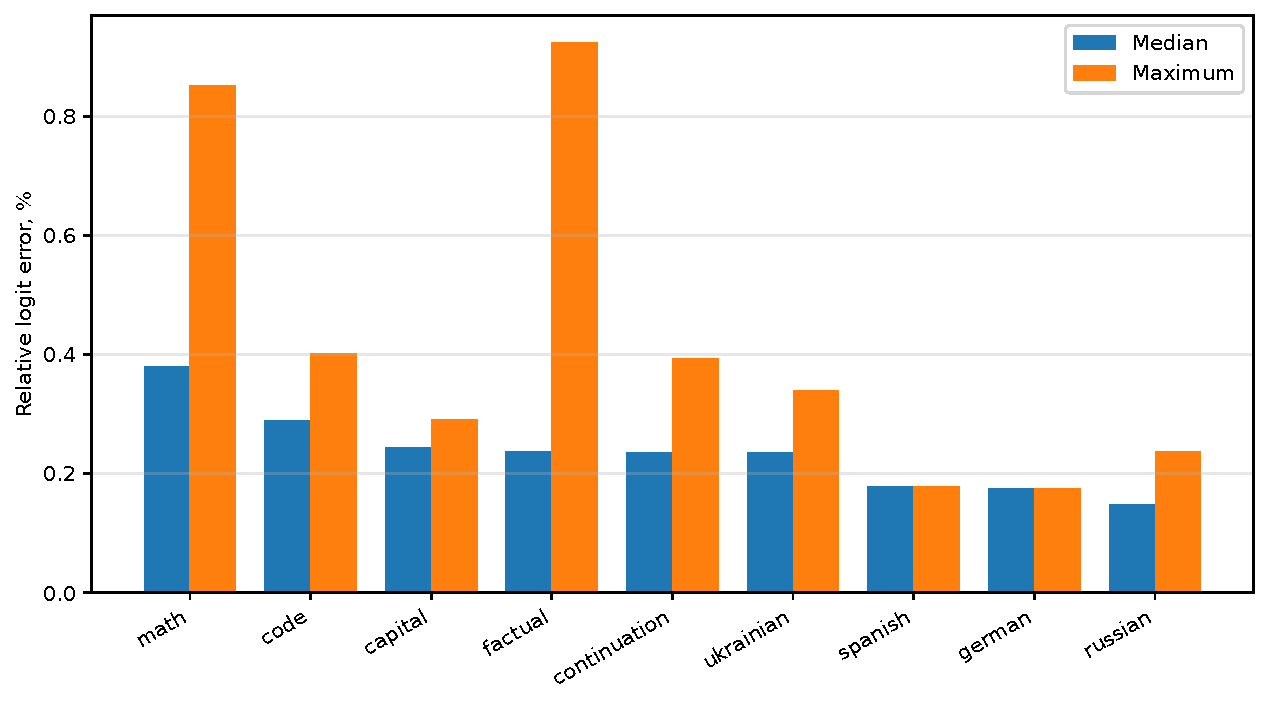
\includegraphics[width=\linewidth]{figures/fig4_global_replacement_by_suite.pdf}
\caption{Error of global attention+MLP backbone replacement by prompt category; bars show the median and maximum within each category.}
\label{fig:prompt-suites}
\end{figure}

\section{Discussion}

\subsection{The central object of the
method}

The central object is not an isolated matrix, but the combination

\begin{align*}
&\text{weight-derived structure} + \text{input-dependent execution} \\
&\qquad + \text{executable replacement} + \text{factorized intervention}.
\end{align*}

The static structures are \(M_{qk}^{aug}[d]\), \(C_{vo}^{aug}\), and
\(B_j\). The dynamic quantities are hidden states, attention
probabilities, and MLP coefficients.

\subsection{Why global replacement is stronger than a local
identity}

An algebraic formula may be correct while an implementation is wrong
about RoPE orientation, normalization placement, head layout, GQA
mapping, masking, or dtype. Global replacement tests the entire chain
simultaneously.

\subsection{Comparison with activation
patching}

Activation patching commonly uses cached clean or corrupted activations.
Here, the component value is \textbf{recomputed} from the current hidden
state through a weight-derived program. This supports faithful
replacement, QK-only intervention, VO-only intervention, and MLP
intervention through one interface. We do not claim that activation
patching is fundamentally incapable of intercepting internal Q/K/V
tensors; the distinction is that our replacement is defined by an exact
program representation rather than a cached counterfactual activation.

\subsection{Preparatory components and distributed
computation}

Delayed downstream peaks are consistent with inter-layer communication
and preparatory components. However, the propagation metric measures
perturbation in the downstream graph as a whole and does not identify
individual causal edges. A natural next step is to combine the program
interface with path patching, path expansion, or subspace tracing.

\subsection{Superposition}

Rank-1 MLP atoms are native computational objects, but they are not
necessarily monosemantic features. This work does not resolve
superposition; an SAE or transcoder can be applied on top of the program
representation as an additional analysis layer.

\section{Related work}

\subsection{Transformer circuits}

Transformer-circuit work~\citep{elhage2021framework} established the language of QK/OV
decomposition, read/write maps, and attention-head analysis. We extend
this line to a faithful extractor for RoPE/RMSNorm/GQA/bias/SwiGLU and
evaluate not only analysis but global executable replacement.

\subsection{Locally linear
mappings}

Detached-Jacobian approaches, particularly Golden~\citep{golden2025locally}, construct nearly
exact input-specific linear maps of a model or component. Our object
differs: structural targets are derived from weights and reused across
inputs, while input-dependent execution remains explicit in attention
probabilities and MLP coefficients.

\subsection{Singular-vector and component
decomposition}

Beyond Components~\citep{ahmad2025beyond} studies singular directions and subfunctions within
attention and MLP components. Our factorization does not compete with
SVD as a method for finding subspaces; it defines a native executable
representation on top of which SVD can be applied.

\subsection{Activation patching and causal
tracing}

Activation patching and causal tracing~\citep{zhang2023patching,heimersheim2024patching} localize causally important
components by replacing activations from other runs or with synthetic
values. We follow the same interventional logic, but replace the
component not with a cached activation, but with a value recomputed
through the weight-derived program on the current hidden state.

\subsection{Causal scrubbing}

Causal scrubbing~\citep{chan2022causal,geiger2023causal} tests interpretability hypotheses by replacing
intermediate values with resampled values consistent with the
hypothesis. Our work is related in spirit to mechanism replacement, but
the replacement object differs: rather than hypothesis-driven
resampling, we use the component's exact weight-derived program. This
gives a narrower but stricter objective: faithful replacement and
factorized intervention for native component computation.

\subsection{Sparse autoencoders and
transcoders}

SAEs construct a learned feature basis over activations~\citep{bricken2023monosemanticity}. Transcoders
train a sparse surrogate for a component, most commonly an MLP, to
approximate its input-output mapping and facilitate circuit analysis.
Our approach does not train a surrogate or take optimization steps: the
program is extracted directly from the weights and achieves a median
replacement discrepancy of \textbf{0.139\%} across all 24 MLPs without
training.

\subsection{Talking Heads and inter-layer
communication}

Work on inter-layer communication~\citep{merullo2024talking} studies low-rank channels through
which information is passed between layers and heads. Our complete atlas
supports the prevalence of delayed downstream effects, but does not
isolate specific communication subspaces.

\subsection{RASP decompilation and white-box
models}

RASP decompilation~\citep{huang2026rasp} extracts symbolic programs from small algorithmic
transformers. White-box architectures~\citep{yu2023whitebox} construct new interpretable
models. We instead analyze a pretrained language model and construct a
matrix, rather than symbolic, program for its native components.

\section{Limitations}

\begin{enumerate}
\def\labelenumi{\arabic{enumi}.}
\tightlist
\item
  Only one model, Qwen2.5-0.5B-Instruct, was evaluated.
\item
  The prompt suite contains 64 short next-token prompts rather than a
  large benchmark.
\item
  We do not report corpus-level perplexity or loss.
\item
  We do not evaluate long contexts or large RoPE distances.
\item
  The program path uses float32 for part of the computation, whereas the
  native model runs in fp16.
\item
  The native identity control for attention is a sanity check rather
  than an independent estimate of a numerical lower bound.
\item
  Propagation measures downstream perturbation, but not individual
  causal edges.
\item
  The held-out atom experiment is not part of the main claims: in the
  original run, three random controls were duplicated because of a seed
  bug; the corrected code is released separately.
\item
  The gate lens remains exploratory and is used only for the qualitative
  illustration.
\item
  We make no claim of inference speedup.
\end{enumerate}

\section{Conclusion}

We presented an executable component-level representation of a
pretrained Qwen2.5 transformer. All attention and MLP computations were
replaced by weight-derived program execution with a median logit error
of \textbf{0.258\%} and \textbf{100\%} top-1 preservation across 64
prompts. The complete head atlas showed that QK and VO interventions
produce effects tens of times larger than the replacement discrepancy,
while MLP interventions produce effects more than one hundred times
larger. Downstream profiles showed that most head effects peak many
layers after the source. A component matrix program is therefore not
only a way to rewrite a formula, but a practical executable interface
for faithful replacement, factorized intervention, and analysis of
distributed computation across model depth.

\appendix
\section{Figure generation}

Figures are generated automatically from the result CSV files with

\begin{verbatim}
python generate_matrix_program_figures_v06_1_fixed.py \
  --results-dir outputs/qwen_matrix_program_final_article_v4/final_article \
  --out-dir figures_v06_1_fixed
\end{verbatim}

The script creates vector PDF and PNG files:

\begin{itemize}
\tightlist
\item
  \texttt{fig1\_method\_overview.pdf}
\item
  \texttt{fig2\_head\_heatmaps.pdf}
\item
  \texttt{fig3\_propagation\_profiles.pdf}
\item
  \texttt{fig4\_global\_replacement\_by\_suite.pdf}
\end{itemize}

\section{Reproducibility}

The minimal GitHub artifact set is:

\begin{itemize}
\tightlist
\item
  the main extractor and patching script;
\item
  the corrected atom-split script with independent random seeds;
\item
  a \texttt{README.md} with the exact run command;
\item
  \texttt{all\_experiment\_summaries.csv};
\item
  \texttt{all\_prompt\_metrics.csv};
\item
  \texttt{head\_causal\_atlas.csv};
\item
  \texttt{mlp\_causal\_atlas.csv};
\item
  \texttt{layer\_group\_atlas.csv};
\item
  \texttt{propagation\_profiles.csv};
\item
  \texttt{experiment\_manifest.json};
\item
  \texttt{final\_prompts.json};
\item
  environment versions and a hardware note.
\end{itemize}


\nocite{*}
\bibliographystyle{plainnat}
\bibliography{references}
\end{CJK*}
\end{document}
